\chapter{Gérer un outil de visualisations de données}

Comme on l’a vu, manipuler la base de données issue du processus de production n’est pas particulièrement aisé. Cela requiert des moyens importants, et une expertise technologique poussée. Or il faut pouvoir donner la possibilité de visualiser les données à certains partenaires du projet, notamment les services d’archives qui n’ont pas ces moyens ou cette expertise. C’est pourquoi il a été décidé de recourir à un outil d’analyse et de visualisation de données, plus simple à manipuler. 

\section{Une base de données, pour qui?}

L’un des objectifs du projet SocFace est de permettre aux services des archives départementaux et municipaux de valoriser leurs fonds documentaires. Comme mentionné précédemment, les listes de recensements sont des ouvrages volumineux et difficiles à manipuler, ce qui incite ces services à s'engager dans le projet. Cependant, les archives ne pourront pas accéder à la base de données finale avant la fin du projet, en 2025. Dans l'intervalle, il est donc essentiel de leur fournir des informations exploitables sur les images qu’ils ont contribué à numériser.\\
SocFace a donc cherché à mettre en place un outil de visualisation des données, qui, bien que limité, permet de donner un aperçu des volumes traités. Contrairement à un système de gestion de base de données classique, cet outil n’a pas pour vocation de faciliter la recherche approfondie, comme la consultation de noms spécifiques ou de communes. Il s'agit plutôt de générer des visualisations synthétiques, telles que des graphiques, des histogrammes ou des diagrammes en camembert, afin de donner une vue d'ensemble des données traitées. Ce type d’analyse légère permet aux services d'archives de suivre l'état d'avancement du projet, en attendant la mise à disposition de la base de données complète, qui sera développée en collaboration avec le SIAF. En parallèle, cet outil sert également les besoins internes du projet SocFace. Lancé il y a deux ans, il est crucial de réaliser des points d’étape réguliers pour évaluer l’avancement et ajuster les efforts si nécessaire. De plus, ces visualisations sont précieuses pour les présentations lors de conférences ou autres événements de valorisation de la recherche, offrant ainsi une meilleure visibilité sur les progrès accomplis. Dans les deux cas, l’objectif est de créer un tableau de bord personnalisé pour chaque département, permettant de suivre l'évolution de la production de leurs données, notamment les mentions (noms, professions, âges, etc.) et les métadonnées (communes, dates, départements). Idéalement, ce tableau de bord sera dynamique et connecté à la base de données de l’INED, offrant ainsi une mise à jour en temps réel de l’état des travaux.

\section{Metabase, un bon choix?}
Afin de réaliser ce tableau de bord, les équipes de SocFace ont choisi la solution offerte par Metabase . C’est un outil de Business Intelligence (\textit{ensemble des outils, des technologies et des méthodes utilisés pour collecter, analyser et présenter des données d'une entreprise. L'objectif est d'aider les décideurs à mieux comprendre les performances de l'entreprise et à prendre des décisions éclairées. En d'autres termes, la BI transforme des données brutes en informations utiles pour guider les stratégies et les actions d'une entreprise}). C’est un outil en open source, ce qui signifie que son code est ouvert et son utilisation autorisée pour tous (sous réserve de respecter la licence sous laquelle le programme est distribué).\\
Metabase fonctionne par connexion à une base de données. C’est très utile pour les bases de données de grande ampleur comme c’est le cas pour SocFace, puisqu’il n’y a pas de téléchargement de la base de données et donc pas de limite au nombre de lignes possibles. Un autre avantage est que les données sont mises à jour automatiquement. Mais cela implique aussi des contraintes techniques, puisqu’il faut avoir un accès au serveur et celui-ci doit être stable.\\
En termes de fonctionnement, Metabase est très intuitif : basé sur les requêtes SQL\footnote{Voir Glossaire}, il permet à des novices, qui ne possèdent pas ce langage, de pouvoir interroger la base de données. Grâce à une interface très simple, l’utilisateur est invité à exprimer son besoin, et le programme transforme sa question en requête SQL, de façon transparente. On peut également indiquer sa propre requête SQL si on maîtrise le langage, pour effectuer des requêtes plus complexes. Une fois les données agrégées en réponse à notre question, on choisit le type de visualisation qui nous convient. Les différentes visualisations sont associées pour créer un tableau de bord. 

\begin{figure}[H]
        \centering
        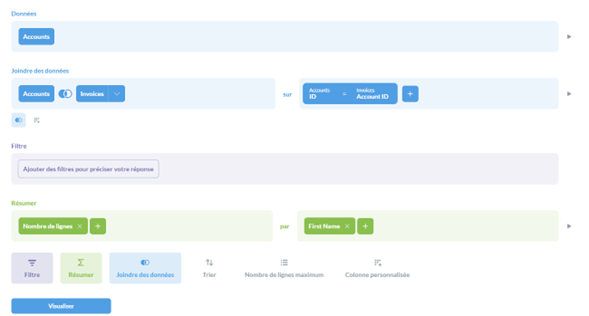
\includegraphics[width=1.0\linewidth]{Figures/Partie 2/Fig.2.2 - Metabase.png}
        \caption[Interface Metabase - Formuler une question]{Interface Metabase - Formuler une question}
        \label{fig:Fig2.2}
    \end{figure}

Concernant le projet SocFace, nous nous en sommes servis pour créer des tableaux de bord pour les premiers départements à avoir intégré la base de données. Les tableaux de bords reprennent uniquement les métadonnées c’est-à-dire les informations sur ce qui est entré dans la base de données, mais pas sur les données elles-mêmes. 
\clearpage

\begin{figure}[H]
        \centering
        \includegraphics[width=0.95\linewidth]{Figures/Partie 2/Fig.2.3 - Metabase - Visualisation pour le Puy-de-Dôme.jpg}
        \caption[ Metabase - Visualisation pour le Puy-de-Dôme]{ Metabase - Visualisation pour le Puy-de-Dôme}
        \label{fig:Fig2.3}
    \end{figure}

Sur cet exemple, nous pouvons ainsi voir : 
\begin{itemize}
    \item Un tableau croisé dynamique sur le nombre de pages traitées, par année et par commune ;
    \item Un tableau croisé dynamique sur le nombre de pages traitées, par année et par commune ;
    \item Le nombre de commune dans le département ;
    \item Le nombre de pages total traité et par année sur un camembert ; 
    \item Le nombre de document traité par année, qui correspond à peu près au nombre de commune puisqu’il y a un document par commune ; 
    \item Le nombre de page traité par année sur un histogramme ;
    \item La comparaison entre le nombre de pages traitées pour le Puy-de-Dôme et les autres départements traités. 
\end{itemize}

Une fois ces tableaux élaborés, l’idée était de les automatiser afin de pouvoir créer ces tableaux pour chacun des départements et qu’ils soient mis à jour en synchronicité. Malheureusement, Metabase ne permet pas cette automatisation. S’il y a une mise à jour sur la base de données, il faut repasser par la procédure de question. Cela nécessiterait donc que chaque service d’archive utilise directement Metabase et crée son propre tableau de bord. Là encore, ce n’est pas possible car Metabase est connecté à un serveur de l’INED qui héberge la base de données. Or on ne peut pas se connecter à ce serveur hors de l’établissement de l’INED au Campus Condorcet, pour des raisons de sécurité. Par ailleurs, le traitement par le programme des questions peut être très long. Lorsque nous avons créé les tableaux de bord « tests », il n’y avait que 24 départements et le temps de chargement des résultats pouvait parfois prendre plus de 3mn. En supposant que les 98 services d’archives qui ont donné leur accord envoient bien leurs images, il va être très difficile d’obtenir de bonnes performances via Metabase. \\

Cet outil était donc adéquat pour les besoins du projet : permettre à des novices en langage \gls{SQL} de pouvoir élaborer des tableaux de bords de suivi du projet. C’était intéressant dans un contexte d’interdisciplinarité car tous les membres du projet ne sont pas compétents en SQL. Dans l’hypothèse où on aurait laissé les services d’archives accéder à l’outil, ils auraient pu générer leurs propres visualisations sans trop de complexité. \\
Il ne sera donc pas retenu pour cette utilisation, mais reste un outil intéressant pour une utilisation interne au projet, et peut servir de supports pour une valorisation du projet lui-même. Il faut simplement admettre qu’il ne pourra pas être automatisé et demandera donc une certaine maîtrise de l’outil par l’utilisateur. 




